\documentclass{article}

% set font encoding for PDFLaTeX, XeLaTeX, or LuaTeX
\usepackage{ifxetex,ifluatex}
\newif\ifxetexorluatex
\ifxetex
  \xetexorluatextrue
\else
  \ifluatex
    \xetexorluatextrue
  \else
    \xetexorluatexfalse
  \fi
\fi

\ifxetexorluatex
  \usepackage{fontspec}
\else
  \usepackage[T1]{fontenc}
  \usepackage[utf8]{inputenc}
  \usepackage{lmodern}
\fi

\usepackage{hyperref}
\usepackage{amsmath}
\usepackage{graphicx}

\title{Kettősinga szimuláció felhasználói dokumentációja}
\author{Nógrádi Zsófia}

% Enable SageTeX to run SageMath code right inside this LaTeX file.
% http://mirrors.ctan.org/macros/latex/contrib/sagetex/sagetex.pdf
% \usepackage{sagetex}

\begin{document}
\maketitle
\pagebreak
\tableofcontents
\pagebreak

\section{A feladat}
A kettősinga kaotikus mozgásának modellezésére íródott a program. A kettős inga két inga egymáshoz csatolásával keletkező egyszerű rendszer,melynek mozgását a kezdeti feltételek erősen befolyásolják. Ez az objektum a legelterjedtebb demonstrációs erszköze a kaotikus mozgásnak.

\section{A fizikai leírása}
Az alap fizikai ismereteinket használjuk fel arra, hogy felírjuk a Newton-féle erőtörtvényeket a rendszerre. A továbbiakban használjuk a következő jelöléseket:

\begin{align*}
x &:  az ingatömeg vízszintes helyzete \\
y &: az ingatömeg függőleges helyzete \\
\theta &: az inga szöge \\
L &: a kötél hossza \\
F &: a kötélerő \\
m &: az ingatömege \\
g &: nehézségi gyorsulás értéke
\end{align*}

Pusztán geometriai tudáunkat elővéve felírjuk az ingatömegek helyzetét: 
\begin{gather*}
x_1=L_1 \sin \theta_1 \\
y_1= - L_1 \cos \theta_1 \\
x_2 = x_1 + L_2 \sin \theta_2 \\
y_2= y_1 - L_2 \cos \theta_2 \\
\end{gather*}

Ezeket az egyenleteket kétszer deriválva megkapjuk a gyorsulás értékét, majd azt felhasználva felírhatjuk a dinamika alaptörvényét, ami alapján $F=m \cdot a$ Az így kapott egyenleteket $\theta ''$-re rendezve adódnak azon differenciálegyenletek, amiket a programunk Runge-Kutta-módszerrel oldja meg. A továbbiakban elsősorban jelölés szempontjából bevezetjük a szögsebességet $\omega $ ami éppen $\theta$ első deriváltja. Így a Runge-Kuttának már négy elsőrendű differenciálegyenletet tudunk átadni, amit az meg tud oldani. Ezek a következőek:
\begin{gather*}
\theta_1' = \omega_1 \\
\theta_2' = \omega_2 \\
\omega_1' = \frac{-g(2m_1+m_2)\sin \theta_1 - m_2\cdot g \cdot \sin(\theta_1-2\theta_2) - 2 \sin(\theta_1 - \theta_2)m_2(\omega_2^2 L_2 + \omega_1^2 L_1 \cos(\theta_1 - \theta_2))}{L_1(2m_1 + m_2 - m_2 \cdot \cos(2\theta_1 - 2 \theta_2))} \\
\omega_2'=\frac{2 \sin(\theta_1 - \theta_2)(\omega_1^2 \cdot L_1(m_1+m_2) + g(m_1+m_2) \cos \theta_1 + \omega_2^2 \cdot L_2 \cdot m_2 \cos(\theta_1-\theta_2))}{L_2(2m_1+m_2-m_2\cos(2\theta_1 - 2 \theta_2))} \\
\end{gather*}

\section{Negyedrendű Runge-Kutta-módszer}
A módszer differenciálegyenletrendszerek megoldására alkalmas. Ahogy azt a neve is sugallja, ez egy negyedrendű közelítő módszer, ahol egy választott pici lépésközhöz n-edik (ahol n tipikus nagy) lépésben oldja meg a kezdetiértékproblémát.

\section{Fejlesztői környezet}
\subsection{Összefoglaló}
A program C++ program nyelven íródott, ami jól fordul CodeBlocks-ban Cmake, vagy C/C++ fordítással, és VisualStudioban is.
\subsection{Microsoft Visual Studio Telepítése Windows rendszerre}
A Visual Studio pár éve ingyenesen letölthető például \url{https://code.visualstudio.com/}
\begin{figure}[h!]
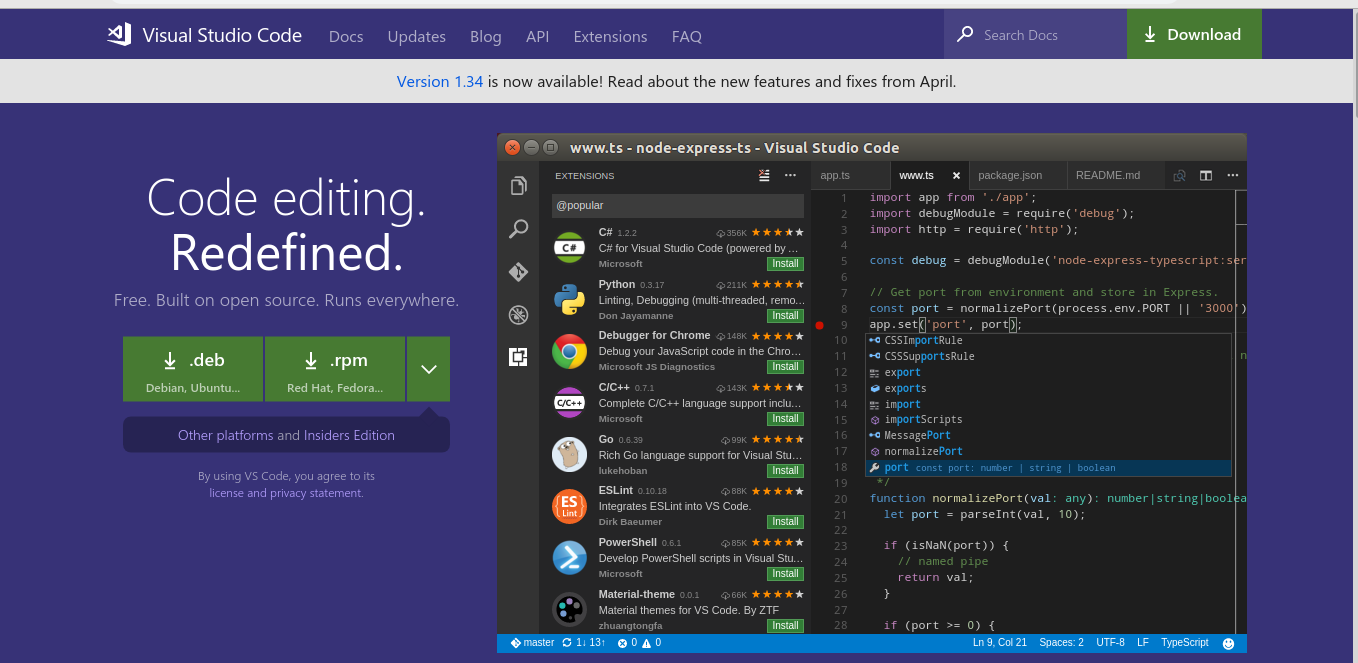
\includegraphics[width=10cm]{screeen.png}
\caption{Telepítő felület}
\end{figure}
A telepítés egyszerűen vezetett telepítés, majd a környezet megnyitásakor még telepítjük rá a CMake-t, a CMake Tools-t és a C/C++-t. Majd Scan for Kits-nél jó eséllyel megakadunk, vagy olyan elavult fordítót találunk, aminek a megléte teljesen felesleges. Szóval még egy fordítót sem árt telepítenünk, ami például lehet: Build Tools for Visual Studio 2019, ami elérhető a \url{https://visualstudio.microsoft.com/downloads/} címről, ha lejjebb görgetünk, akkor azonnal megtaláljuk a fentebb említett fordítót, amit szintén egyszerűen tudunk telepíteni. Ha ez megvan újra rámegyünk a Scan for Kitsre és kivlasszuk a telepített fordítót, ha sikerült azt a path-ban elhelyezni, hanem, akkor hibaüzenetet kapunk, aminek megoldása az, hogy megkeressük a path mappát és áthelyezzük oda a fordítót. 

\subsection{Microsoft Visual Studio problémák}
A telepítés nem volt éppen egyszerű, hiszen az egyik operációs rendszerem, a Linux családba tartozó Endless csodálatos biztonsági rendszere csak a saját Appstore-ból való telepítést engedélyezte. Ezzel még nem is volt feltétlen baj, a VS Code itt is elérhető volt, viszont a fordítója egy őskövületnél megállt, így alkalmatlanná vált arra, hogy használni tudjam. Tehát a későbbiekben arra kényszerűltem, hogy a Windows 8-cas rendszerű, kevéssé alkalmas gépemre telepítsem a VS Code-ot és a magát a fordítót. Ez sem volt leányálom, ugyanis a fordítót csak nem akarta elérhetővé tenni a Path-nak, majd sok újratöltést követően sikerült a path-ban elhelyezni a fordítót. Ami van két hétig jól viselte ott magát, majd a gép egy frissítése során nem ismerte fel a környezet, így kezdődött az egész előlről. Jelenleg működőképes a program.

\section{Kezdetek}
Először egy Git repozitóriumot kellett nyitni a Githubon.
\begin{figure}[h!]
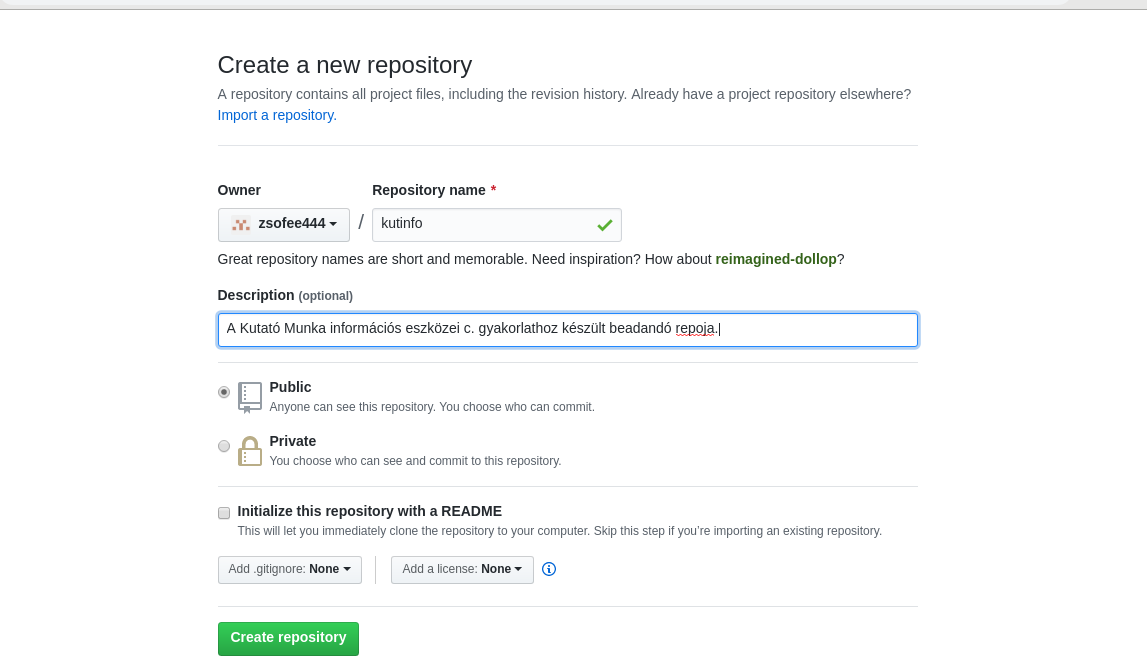
\includegraphics[width=10cm]{git.png}
\caption{Git repo létrehozása}
\end{figure}
Majd a Visual Studioban klónozzuk a repo-t a Git-re, hogy a programírás minden metódusa bekerüljön. 

\section{A program használata}
Két fontos részből épül fel a projekt. Az egyik a "miniwindow.h" ez a tárgy oktatói által megírt ablakkezelő header, ami elérhető a nyilvános GitHub-ról \url{https://github.com/u235axe/miniwnd} címről. Ez a program teszi lehetővé a kettősinga kirajzolását és a mozgatását is. 
A másik rész az maga a "main.cpp", ahol igazából az érdemi része történik a programnak. Először egy 4 komponensű pici vektorstruktúra megírása látszik, amiben csak azok a műveletek vannak definiálva, amire a differenciálegyenlet megoldása során szükségünk lesz, tehát a szorzár, összeadás illetve a skalárral való osztás.
\newline
Ezután következik a Runge-Kutta metódus definiálása, majd a rajzoltatás kezdeti fázisai az App struktúrában. Megadjuk a kezdeti értékeket, az ingatestek tömegét az ingák osszát, a nehézségi gyorsulás értékét, a Runge-Kutta-módszer léptetésének hosszát, a kezdeti időt és a kezdeti értéket. A négyesvektor felépítése végig: $(\theta_1, \theta_2, \omega_1, \omega_2)$. 
\begin{itemize}
\item wnd.mouseHandler az egérrel való műveletek elvégzését végzi. Erre most nincs szükségünk, így ezt nem kell babrálni.
\item wnd.resizeHandler az ablak újraméretezésekor fellépő műveletek elvégzését végzi. Most ez is alapbeállításon marad.
\item wnd.idleHandler-ben hívjuk meg a Runge-Kutta metódust, mostmár a négykomponensű vectorunkba beírva a differenciálegyenleteket, amiket az algoritmus megad. 
\item wnd.renderHandler akkor hívódik meg, amikor az ablak újrarjzolódik. Itt adjuk meg a pixelek alap színét, és a két ingatestből és két fonálból álló rendszer kooridnátáit. És azok változását az időben.
\item wnd.open pedig magát az ablakot formázza, megadja, hogy hol és mekkora méretben nyíljon meg, hogy mi legyen az ablak neve és hogy az ablak rendelkezzen a három alap funkcióval is. 
\end{itemize}
Az így megírt App függvényt hívjuk be a main-be, hogy működjön a program. 

\section{Akadályok}
A probléma az volt elsősorba, hogy a VS Code nem akarta az igazságot, így elkeseredésemben a CodeBlocksal és netes fordítókkal próbálkoztam. A netes fordítókon azonban a "miniwindow.h" különböző alap package-ei hiányoztak, így azok hamar kiestek a próbálkozásból. Majd a sok próbálkozás után ugye a klónozést a VS Code-dal történt, ezért semmire nem jutottam a CodeBlockssal. De végül segítséggel a VS Code használhatóvávált. 
A nehézséget főleg az ablakkezelő parancsok okozták, mivel ezek teljesen újak voltak, de sokat segített a tanárok által előre megírt Lotka-Volterra szimuláció, amit az egész alapjául vettem.
\end{document}
